% Introdução
\chapter*{Introdução}

Segundo a Organização das Nações Unidas \cite{un2010state}, em 2050, 91,4\% da população da América Latina viverá em áreas urbanas. Assim como em outros países, se agravam no Brasil os problemas decorrentes do aumento da densidade demográfica nos centros urbanos. Poluição, epidemias, congestionamentos, violência e outros problemas têm se tornado uma questão urgente para os gestores dos espaços urbanos.  A poluição atmosférica, por exemplo, agravada com o aumento do número de veículos, é responsável por cerca de 20 mil óbitos por ano no Brasil \cite{arbex2012poluiccao}. O aumento do número de veículos é outro problema que vem tomando grandes proporções nas grandes cidades. Como pode ser visto na Figura \ref{fig:crescimentoveiculos}, esse problema tem se agravado especialmente a partir do ano de 2001 \cite{INCT2013evoluccao}.

\begin{figure}[ht]
\centering
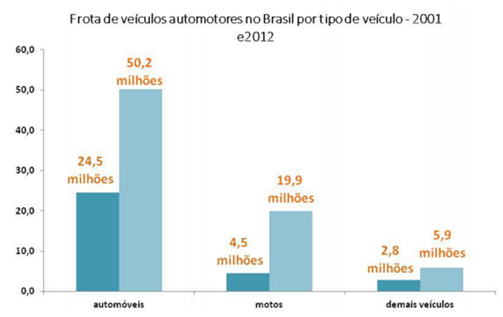
\includegraphics[width=4.5in]{Imagens/carrosUp.png}. 
\caption{Crescimento de veículos no Brasil}
\label{fig:crescimentoveiculos}
\end{figure}

Nesse período, por exemplo, o crescimento do número de veículos nas regiões metropolitanas brasileiras foi de no mínimo 73,1\% (valor alcançado pelo Rio de Janeiro), e mais que dobrou em casos como Curitiba, Belém e outras, como é possível observar na Figura \ref{fig:crescimentocarros}. Isso indica que o crescimento do número de veículos está acontecendo com valores relativamente altos, e que é necessário ter formas de oferecer respaldo para as iniciativas que tentem lidar com o grande número de veículos e problemas decorrentes.

\begin{figure}[ht]
\centering
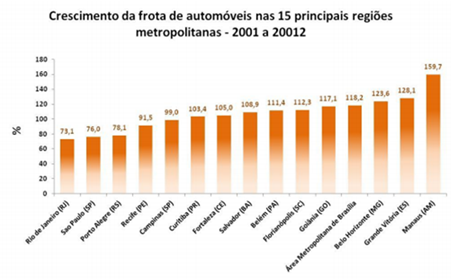
\includegraphics[width=4.5in]{Imagens/carrosUpBrasil.png}.  
\caption{Crescimento de carros nas regiões metropolitanas}
\label{fig:crescimentocarros}
\end{figure}

Ainda nas grandes regiões metropolitanas é possível observar que, em grande parte dos casos, o desenvolvimento urbano não acontece de forma sustentável \cite{rolnik2011crescimento} e não consegue acompanhar demandas urgentes como a necessidade de transporte para pessoas que vive nas metrópoles. Esse fato, aliado ao crescente número de pessoas, acaba transformando o ambiente urbano num plano ideal para o agravamento mais acelerado dos problemas locais. Parte desses problemas se relaciona de forma estreita com os veículos utilizados diariamente pelas pessoas.

Segundo a Wharton School (2013)\cite{WHARTON2013}, cerca de 6 a 7 bilhões de reais de prejuízo foram causados em todo o Brasil, apenas pelos acidentes envolvendo veículos no ano de 2013. Tais prejuízos financeiros se somam a tantos outros problemas, como por exemplo: os ambientais, devido à grande quantidade de poluentes lançados no ambiente; transtornos psicológicos nas pessoas envolvidas em acidentes com veículos; na produtividade, devido à grande quantidade de tempo desperdiçado com problemas de infraestrutura, trânsito ou nos próprios veículos, e etc. Com isso fica claro que o acúmulo de veículos traz consigo uma grande quantidade de problemas, dessa forma é importante pensar em abordagens que possam reduzir ou eliminar tais problemas.

Motivados pelos problemas relacionados acima e com o objetivo de oferecer uma forma de auxiliar no melhor uso de veículos, alguns trabalhos recentes \cite{zhang2016driver,amsalu2016driver,meseguer2015assessing,eren2012estimating}, têm focado em abordagens que permitem a criação de perfis automáticos de usuários (motoristas) de automóveis. Os resultados desses trabalhos possibilitam entender como um motorista utiliza o seu veículo, o que pode trazer benefícios relacionados à eficiência energética, infraestrutura das cidades, seguridade automotiva, planejamento urbano e etc. Neste artigo será abordado o atual estado do uso de técnicas de Aprendizado de Máquina (AM) para a definição de perfis de utilização de veículos e também, proposta uma abordagem para essa forma de descoberta de perfis de motoristas.

O restante deste artigo está organizado da seguinte forma. Em seguida, a Seção XXXXX aborda os trabalhos relacionados à descoberta de perfis de utilização de automóveis, mostrando os aspectos gerais e também aspectos mais específicos dos principais artigos. A Seção XXXXX propõe uma abordagem de solução do problema em questão e faz uma breve contextualização de suas características com o que foi abordado na seção XXXXXX. Por fim, a Seção XXXXX aborda os resultados que se quer atingir com a abordagem proposta.

\section{Organização do trabalho}

Nesta seção deve ser apresentado como está organizado o trabalho, sendo descrito, portanto, do que trata cada capítulo.